\documentclass{beamer}
\usepackage[utf8]{inputenc}
\usepackage[spanish]{babel}
\graphicspath{/images}
\usepackage{graphicx,hyperref,ru,url}

\usepackage{listings}

\title[]{Geometría y visualización}
\subtitle{}
\author[Jesús Bueno Urbano]{Jesús Bueno Urbano\\\medskip{Directores:\\Pedro A. García Sánchez\\Carlos Ureña Almagro}}
\institute[Universidad de Granada]{Trabajo Fin de Máster\\Máster en Matemáticas}
\date[21/09/2018]{21 de septiembre de 2018}

\begin{document}

\begin{frame}
  \titlepage
\end{frame}

\begin{frame}
  \frametitle{Índice}
  \tableofcontents
\end{frame}

\section{Implicitación de superficies}

\begin{frame}{Método de la base de Gröbner}
\begin{equation}
    \begin{tabular}{c c c}
        $x_1$ & = & $f_1(t_1, \dotso, t_m)$, \\
         & $\vdots$ & \\
        $x_n$ & = & $f_n(t_1, \dotso, t_m).$
    \end{tabular}
    \nonumber
\end{equation}
Donde $f_1, \dotso, f_n$ son polinomios en $K[t_1, \dotso, t_m]$ con $K$ un cuerpo.
\pause

Este sistema se puede ver como $F : K^m \to K^n$ definido por
$$F(t_1,\dotso, t_m) = (f_1(t_1,\dotso, t_m), \dotso, f_n(t_1,\dotso, t_m)).$$
\pause
Resolver el problema de pasar a ecuaciones paramétricas a implícitas equivale a encontrar la variedad mínima que contiene a $F(K^m)$. Véase calculando la base de Gröbner reducida del ideal $\langle x_1 - f_1, \dotso, x_n - f_n \rangle$ y encontrando el elemento que no depende de las variables $t_i$.
\end{frame}

\begin{frame}{Metodo de la base de Gröbner}
\textbf{EJEMPLO}
\begin{equation}
\begin{tabular}{c c l}
$x$ & $=$ & $r \cos u \cos t + R \cos t$ \\
$y$ & $=$ & $r \cos u \sin t + R \sin t$ \\
$z$ & $=$ & $r \sin u$
\end{tabular}
\nonumber
\end{equation}
\pause

\begin{equation}
\begin{tabular}{r c c}
$x - r c_u c_t - R c_t$ & $=$ & $0$ \\
$y - r c_u s_t - R s_t$ & $=$ & $0$ \\
$z - r s_u$ & $=$ & $0$
\end{tabular}
\nonumber
\end{equation}
\pause

\begin{equation}
\begin{tabular}{r c c}
$c_u^2 + s_u^2 - 1$ & $=$ & $0$ \\
$c_t^2 + s_t^2 - 1$ & $=$ & $0$
\end{tabular}
\nonumber
\end{equation}
\pause

$$(x^2 + y^2 + z^2 - r^2 - R^2)^2 = 4 R^2 (z^2 - r^2)$$
\end{frame}

\begin{frame}{Método de la resultande de Sylvester}
$f = a_n x^n + \dots + a_0$ y $g = b_m x^m + \dots + b_0$ donde $a_n, b_m \neq 0$
\pause

$$\operatorname{Res}(f,g) = \operatorname{Det}(\operatorname{Syl}(f,g))$$
Donde $\operatorname{Syl}(f,g)$ denota
\small
	$$\begin{pmatrix}
	a_n & & & & & b_m & & & & \\
	a_{n-1} & a_n & & & & b_{m-1} & b_m & & & \\
	a_{n-2} & a_{n-1} & a_n & & & b_{m-2} & b_{m-1} & b_m & & \\
	\vdots & \vdots & & \ddots & & \vdots & \vdots & \vdots & \ddots & \\
	a_1 & \dotso & \dotso & \dotso & a_{n} & b_1 & \dotso & \dotso & \dotso & b_{m} \\
	a_0 & \dotso & \dotso & \dotso & a_{n-1} & b_0 & \dotso & \dotso & \dotso & b_{m-1} \\
	 & a_0 & \dotso & \dotso & a_{n-2} & & b_0 & \dotso & \dotso & b_{m-2} \\
	 & & \ddots & \vdots & \vdots & & & \ddots & \vdots & \vdots \\
	 & & & a_0 & a_1 & & & & b_0 & b_1 \\
	 & & & & a_0 & & & & & b_0
	\end{pmatrix}$$
\end{frame}

\begin{frame}{Método de la resultande de Sylvester}
\textbf{EJEMPLO}
	$$f = x^2 y - 1 \hspace{2cm} g = x^2 + y^2 + xy - 4$$
\pause
	$$\operatorname{Res}(f,g) = \operatorname{Det} \begin{pmatrix}
	y & 0 & 1 & 0 \\
	0 & y & y & 1 \\
	-1 & 0 & y^2 - 4 & y \\
	0 & -1 & 0 & y^2 - 4
	\end{pmatrix}$$ $$= y^6 - 8y^4 + y^3 + 16y^2 - 8y + 1$$
\pause
	$$\langle x - 4y^5- y^4 + 32y^3 + 4y^2 - 64y + 16 , y^6 - 8y^4 + y^3 + 16y^2 - 8y + 1 \rangle$$
\end{frame}

\section{Representación y visualización de superficies implícitas}

\begin{frame}{Triangulación de superficies}
	\begin{figure}[h]
	\centering
	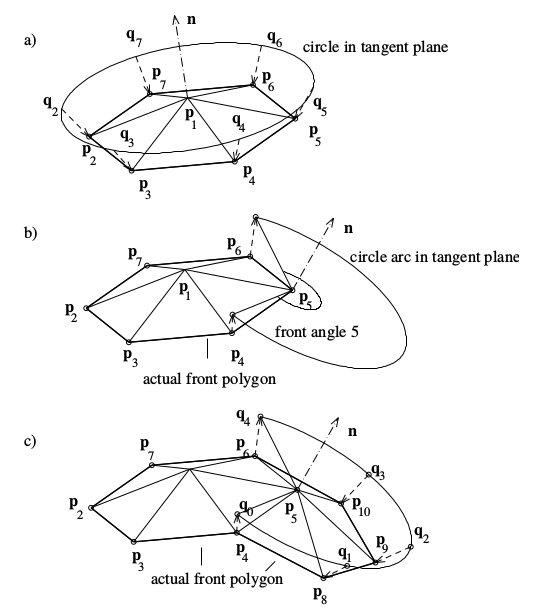
\includegraphics[scale=0.3]{images/hartmann3.png}
	\end{figure}
\end{frame}

\begin{frame}{Triangulación de superficies}
	\begin{figure}[h]
	\centering
	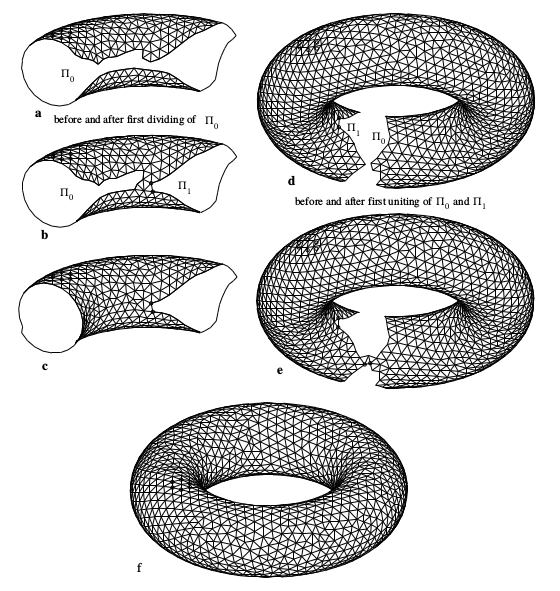
\includegraphics[scale=0.3]{images/hartmann8.png}
	\end{figure}
\end{frame}

\begin{frame}{Ray Tracing}
	\begin{figure}[h]
	\centering
	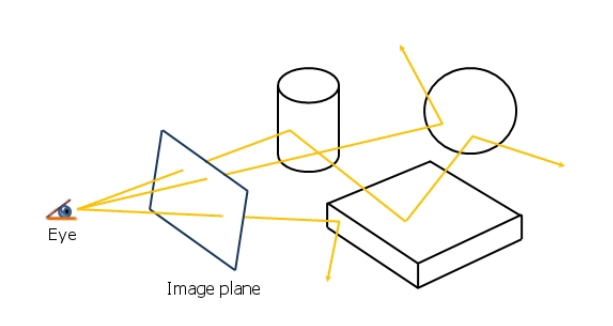
\includegraphics[scale=0.25]{images/florez1.png}
	\end{figure}
\pause
	\begin{figure}[h]
	\centering
	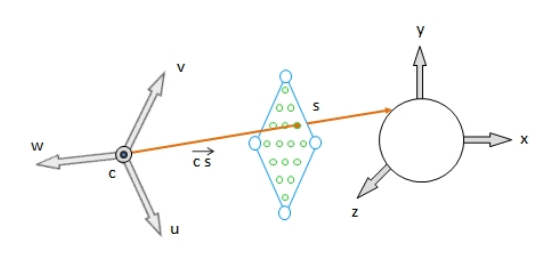
\includegraphics[scale=0.25]{images/florez2.png}
	\end{figure}
\pause
\small
$$g(t) = f(c_x + t(x_s - c_x),c_y + t(y_s - c_y),c_z + t(z_s - c_z))$$
\end{frame}

\section{Análisis de Intervalos}
\begin{frame}{Análisis de Intervalos}
	Una extensión de una función de $\mathbb{R}^n$ a $\mathbb{R}$ dada por $z = f(x_1, \dotso, x_n)$ es el intervalo de extensión unida $R_f$ de $f$. Para el intervalo $X' = (X_1',\dotso, X_n') \in I(\mathbb{R}^n)$ se define el rango de $f$-valores en $X'$ como
	\begin{equation}
	R_f(X_1',\dotso, X_n') := \{ f(x_1, \dotso, x_n) : x_i \in X_i' \ \forall i \in \{1, \dotso, n \} \}
	\nonumber
	\end{equation}
\pause
	\begin{equation}
	f^*(X) := \left[ \min_{x_p \in X_p'} \max_{x_i \in X_i'} f(x_p,x_i), \max_{x_p \in X_p'} \min_{x_i \in X_i'} f(x_p,x_i) \right]
	\nonumber
	\end{equation}
	\begin{equation}
	f^{**}(X) := \left[ \max_{x_p \in X_p'} \min_{x_i \in X_i'} f(x_p,x_i), \min_{x_p \in X_p'} \max_{x_i \in X_i'} f(x_p,x_i) \right]
	\nonumber
	\end{equation}
\end{frame}

\section{Aplicaciones del Análisis de Intervalos y conclusión}
\begin{frame}[fragile]{Aplicaciones del Análisis de Intervalos}
\begin{verbatim}
Evaluate(X,Y,Z):
   If(0 belongs to F(X,Y,Z))
      If(X or Y or Z <= Threshold)
         Add (X,Y,Z) to solution list
      Else
         Subdivide X into X_1 and X_2
         Subdivide Y into Y_1 and Y_2
         Subdivide Z into Z_1 and Z_2
         Evaluate (X_i,Y_j,Z_k) for i,j,k in {1,2}
   Else
      The octant is rejected
\end{verbatim}
\end{frame}

\begin{frame}[fragile]{Aplicaciones del Análisis de Intervalos}
\scriptsize
\begin{verbatim}
Mitchell(T as [t_1,t_2]):
   If(0 in F(T))
      If(0 not in F'(T))
         If(f(t_1)*f(t_2) <= 0)
            Root refinement over T using Bisection or Newthon method
         Else
            T_1 = [t_1,(t_1 + t_2)/2]
            T_2 = [(t_1 + t_2)/2,t_1]
          
            If(width(T_1) >= threshold)
               Mitchell(T_1)
            Else
               Root refinement over T_1 using Bisection or Newthon method
         
            If(width(T_2) >= threshold)
               Mitchell(T_2)
            Else
               Root refinement over T_2 using Bisection or Newthon method
       Else
         Reject T
\end{verbatim}
\end{frame}

\begin{frame}[fragile]{Aplicaciones del Análisis de Intervalos}
\tiny
\begin{verbatim}
Newton(T as [t_1,t_2]):
   If(0 in F(T))
      If(0 not in F'(T))
         t_m = t_1 + midpoint(T)
         NT = t_m - f(t_m)/F'(T)
         NTT = NT intersecting with T
        
         If(NTT is empty)
            There's no root
         Else
            Newton(NTT)
        
      Else
         T_1 = [t_1,midpoint(T)]
         T_2 = [midpoint(T), t_2]
         
         If(width(T_1) >= Threshold)
            Newton(T_1)
         Else
            T_1 is the root
            
         If(width(T_2) >= Threshold)
            Newton(T_2)
         Else
            T_2 is the root
   Else
      Reject T
\end{verbatim}
\end{frame}

\begin{frame}{Aplicaciones del Análisis de Intervalos}
\begin{figure}[h]
\centering
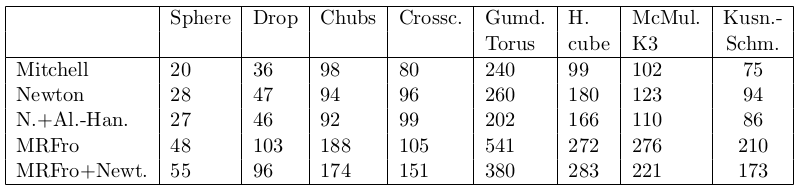
\includegraphics[scale=0.3]{images/florez7.png}
\end{figure}
\begin{figure}[h]
\centering
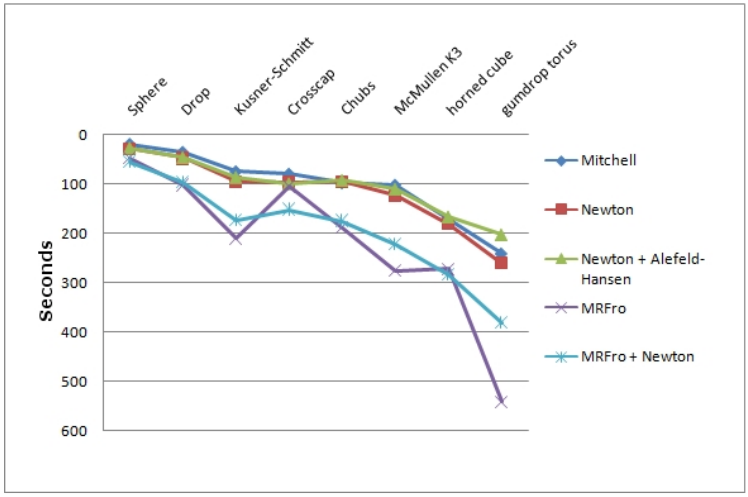
\includegraphics[scale=0.25]{images/florez8.png}
\end{figure}
\end{frame}

\begin{frame}{Bibliografía}
    \tiny
    \nocite{*}
    \bibliographystyle{alpha}
    \bibliography{references}
\end{frame}

\end{document}
